%!Tex Root = ../Tutorat2.tex
% ./Packete.tex
% ./Design.tex
% ./Deklarationen.tex
% ./Aufgabe1.tex
% ./Aufgabe2.tex
% ./Bonus.tex

\section{Task 3}

\setcounter{task}{1}

\begin{frame}[allowframebreaks]{Task 3}{Bonus Practice\vspace{0.5cm}}
  \begin{itemize}
    \item We see from the table that the period P is 30, and we can use 3 as the frame f. Since this task set is a small one, we can derive a feasible schedule graphically...
    \begin{itemize}
      \item \alert{Task 1:} $2f-gcd(15, f)\le 3$  and $f\in\{2, 3, 5, 6\}$
      \begin{itemize}
        \item $f=2$: $4-1\le 3$ $\checkmark$
        \item $f=3$: $6-3\le 3$ $\checkmark$
        \item $f=5$: $10-5\le 3$
        \item $f=6$: $12-3\le 3$
      \end{itemize}
      \item \alert{Task 2:} $2f-gcd(10, f)\le 5$  and $f\in\{2, 3\}$
      \begin{itemize}
        \item $f=2$: $4-2\le 5$ $\checkmark$
        \item $f=3$: $6-1\le 5$ $\checkmark$
      \end{itemize}
      \item \alert{Task 3 and 4:} $2f-gcd(6, f)\le 5$  and $f\in\{2, 3\}$
      \begin{itemize}
        \item $f=2$: $4-2\le 5$ $\checkmark$
        \item $f=3$: $6-3\le 5$ $\checkmark$
      \end{itemize}
    \end{itemize}
  \end{itemize}
  \begin{figure}
    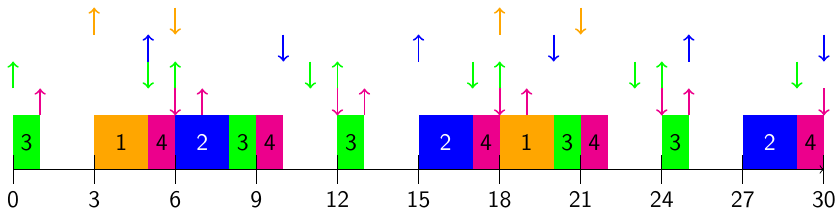
\includegraphics[width=0.7\paperwidth]{./figures/task3_schedule.png}
    \caption{Schedule for Task 3}
  \end{figure}
\end{frame}
